\section*{3. 原子の構造と同位体}
\begin{minipage}{0.55\textwidth}
\begin{enumerate}
    \item 右図は原子の構造モデルである。図の(A)～(D)が示す粒子の名称を答えなさい。\\[0.2cm]
    (A)（ \hspace{4cm} ）\\
    (B)（ \hspace{4cm} ）\\
    (C)（ \hspace{4cm} ）\\
    (D)（ \hspace{4cm} ）
    \item 原子が全体として電荷を帯びていない（電気的に中性である）理由を簡潔に答えなさい。\\[0.2cm]
    理由（ \hspace{10cm} ）
    \item 原子番号が同じで、中性子の数が異なる原子同士を互いに何というか。\\[0.2cm]
    （ \hspace{5cm} ）
\end{enumerate}
\end{minipage}
\begin{minipage}{0.4\textwidth}
\begin{center}
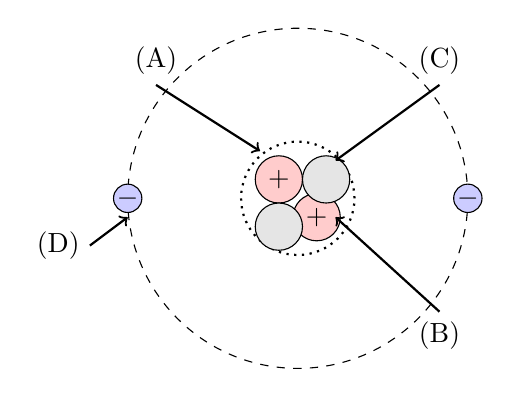
\begin{tikzpicture}[scale=1.2]
    % 電子の軌道
    \draw[dashed] (0,0) circle (1.8);
    % 原子核（全体を囲む円）
    \draw[dotted, thick] (0, 0) circle (0.6);
    % 陽子と中性子
    \draw[fill=red!20] (-0.2, 0.2) circle (0.25) node {$+$};
    \draw[fill=red!20] (0.2, -0.2) circle (0.25) node {$+$};
    \draw[fill=gray!20] (0.3, 0.2) circle (0.25);
    \draw[fill=gray!20] (-0.2, -0.3) circle (0.25);
    % 電子
    \draw[fill=blue!20] (1.8,0) circle (0.15) node {$-$};
    \draw[fill=blue!20] (-1.8,0) circle (0.15) node {$-$};
    % 引き出し線
    \draw[->, thick] (-1.5, 1.2) node[above] {(A)} -- (-0.4, 0.5);
    \draw[->, thick] (-2.2, -0.5) node[left] {(D)} -- (-1.8, -0.2);
    \draw[->, thick] (1.5, -1.2) node[below] {(B)} -- (0.4, -0.2);
    \draw[->, thick] (1.5, 1.2) node[above] {(C)} -- (0.4, 0.4);
\end{tikzpicture}
\end{center}
\end{minipage}
